% Chapter Template

\chapter{Literature Review} % Main chapter title

\label{Chapter2} % Change X to a consecutive number; for referencing this chapter elsewhere, use \ref{ChapterX}

%----------------------------------------------------------------------------------------
%	BACKGROUND
%----------------------------------------------------------------------------------------

\section{Background}

My thesis aims to investigate a form of task automation which links the technologies of the Internet of Things (IoT) and unmanned micro aerial vehicles (MAVs). These topics span across many disciplines, ranging from telecommunications to aeronautical engineering. Therefore, it is important that previous and current research in these areas is sufficiently reviewed before undertaking my own research.

%-----------------------------------
%		AUTOMATION
%-----------------------------------
\subsection{Automation}

Currently, automation in the future workforce is in the eye of the public and at the forefront of much innovation, policy and research (Edmonds 2015). Amongst other factors, the relative cost and unreliability of human workers when compared to computers is driving companies to automate operations. Recent examples range from the transport and logistics of goods (CNET 2014) to the synthesis of written media content (Smith 2015). According to CEDA (2015), 39.6\% of the current jobs in Australia have a high probability of ‘computerisation’. Autor, Levy and Murnane (2003) argue that “computer capital substitutes for workers in performing cognitive and manual tasks that can be accomplished by following explicit rules”.

%-----------------------------------
%		TELEMETRY
%-----------------------------------

\subsection{Telemetry}
The word, ‘telemetry’ is made up the components ‘tele-’ meaning ‘far off, afar, at or to a distance’ and ‘-metry’ meaning ‘meter, measure, or measurement’. Therefore, it involves the measurement of a physical quantity from a location different to that of the source. This practice has been around for almost 100 years, with (Linder 1929) outlining the then current methods of “telemetering” and supervisory control of energy generation, transmission and distribution. In many other applications, being able to quantify parameters of a system remotely is crucial to the system functioning properly.

One such telemetry task that has already begun to be automated is meter reading. In 2013, an Australian company, Taggle, reports that they have deployed a low-power WAN consisting of more than 100,000 motes with customers across the country (Taggle 2016). Their primary product is an internet-connected water meter able to be retrofitted to existing water meters. This solution employs the GSM cellular network, used primarily for voice and data signals of mobile phones, to transfer data from sensors to the internet.

However, there may be sensors embedded in many other forms of infrastructure that don’t have access to the cellular mobile network due to their remote location.

%----------------------------------------------------------------------------------------
%	THE INTERNET OF THINGS
%----------------------------------------------------------------------------------------

\section{The Internet of Things}

Wireless sensor networks (WSNs) form the back-bone of the Internet of Things. According to the IEC (2016), “A wireless sensor network is a network formed by a large number of sensor nodes where each node is equipped with a sensor to detect physical phenomena such as light, heat, pressure, etc.”.

However, the IoT is much more than just hardware. In 1999, Kevin Ashton is believed to have been the first to use the term Internet of Things (IoT). He explained that his intended meaning was about connecting physical things to the digital world, as is only natural for physical people (Ashton 2009). Rose (2014) describes the connected nature of these things as making them “enchanted”. He explains that the idea of “enchanted objects” speaks of the emergence of ordinary things which have extra-ordinary capabilities. Some examples given include a mirror that can aid one’s fashion decisions in a store, an umbrella that knows the weather forecast, or a garbage bin that makes suggestions.

Therefore, it is important to understand where this research topic fits in the scheme of the Internet of Things. Even though a full-stack solution will not be developed, the experimental prototype hardware connects physical quantities to the digital realm. This is the first step to creating an IoT solution.

%----------------------------------------------------------------------------------------
%	MICRO AERIAL VEHICLES
%----------------------------------------------------------------------------------------

\section{Micro Aerial Vehicles}

Micro aerial vehicles (MAVs), or drones as they are referred to in the media, have been used for many novel applications – ranging from disaster relief to taking remote-control selfies (Lily Robotics 2015). They come in many varieties which generally fall under two categories: rotary- and fixed-wing.

%----------------------------------------------------------------------------------------
%		ROTARY WING
%----------------------------------------------------------------------------------------

\subsection{Rotary Wing}

Recently there has been explosion of rotary-wing type platforms, multi-rotors, popping up on crowd-funding platforms such as Kickstarter, and Indiegogo with many a novel and not-so-novel application. These platforms are traditionally used for short and fast flights where the ability to hover in-place and perform a vertical take-off and landing (VTOL) are essential.

%----------------------------------------------------------------------------------------
%		FIXED WING
%----------------------------------------------------------------------------------------

\subsection{Fixed Wing}

Fixed-wing platforms are less nimble, but far more stable and have incredible endurance relative to their hovering counterparts (Wasnak 2001).

%----------------------------------------------------------------------------------------
%	WIRELESS SENSOR NETWORKS
%----------------------------------------------------------------------------------------

\section{Wireless Sensor Networks}

This section outlines the different types of wireless sensor network topologies and challenges facing WSNs. The information contained in this section is adapted from Chapter 4: Sensor Network Topologies and Design Considerations of the book Sensor Technologies: Healthcare, Wellness and Environmental Applications (McGrath 2013).

%----------------------------------------------------------------------------------------
%		NETWORK TOPOLOGIES
%----------------------------------------------------------------------------------------

\subsection{Network Topologies}

A topology can be defined as the way in which constituent parts are interrelated or arranged. For WSNs, a network topology denotes the way in which motes are connected. Many different topologies have been developed for wireless sensor networks, with many resembling those of their previously wired counterparts. Each have their respective strengths and weaknesses. The following subsections briefly explain the 3 most relevant network topologies to the research topic.

%----------------------------------------------------------------------------------------
%		STAR
%----------------------------------------------------------------------------------------

\subsubsection{Star}

The star topology is named after the shape it creates when drawn as a 2-dimensional diagram. This approach relies solely on an intelligent central node sharing point-to-point connections with all other nodes. When implemented, this node is often considered the master device and all others are treated as slave devices.

\begin{figure}[h]
\centering
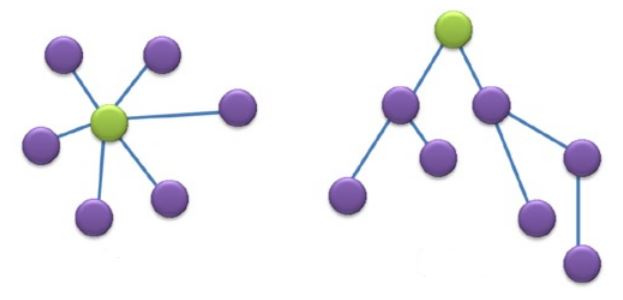
\includegraphics{Figures/star-tree-topology.JPG}
\decoRule
\caption[Star and tree network topologies]{Diagrams of star (left) and tree (right) topologies (McGrath 2013)}
\label{fig:StarTreeTopology}
\end{figure}

Bluetooth and Wi-Fi (IEEE 802.11) are examples of technologies which utilise a star topology, with a smartphone or a wireless router playing the role of the central node and gateway.

%----------------------------------------------------------------------------------------
%		TREE
%----------------------------------------------------------------------------------------

\subsubsection{Tree}


%----------------------------------------------------------------------------------------
%		MESH
%----------------------------------------------------------------------------------------

\subsubsection{Mesh}

The star topology is named after the shape it creates when drawn as a 2-dimensional diagram. This approach relies solely on an intelligent central node sharing point-to-point connections with all other nodes. When implemented, this node is often considered the master device and all others are treated as slave devices.

\begin{figure}[h]
\centering
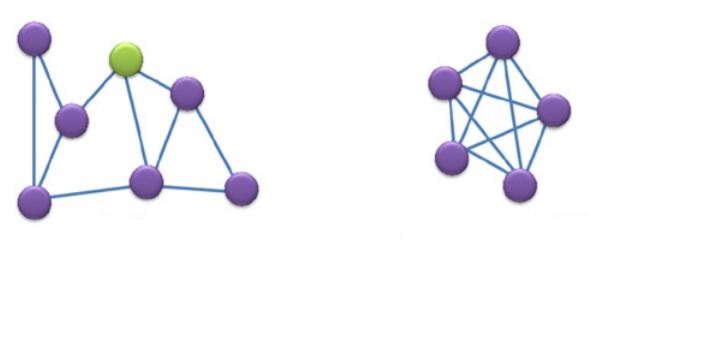
\includegraphics{Figures/mesh-fully-connected-mesh-topology.JPG}
\decoRule
\caption[Mesh and fully-connected mesh network topologies]{Diagrams of mesh (left) and fully-connected mesh (right) topologies (McGrath 2013)}
\label{fig:StarTreeTopology}
\end{figure}

Bluetooth and Wi-Fi (IEEE 802.11) are examples of technologies which utilise a star topology, with a smartphone or a wireless router playing the role of the central node and gateway.

%----------------------------------------------------------------------------------------
%		FULLY-CONNECTED MESH
%----------------------------------------------------------------------------------------

\subsubsection{Fully-Connected Mesh}


